\documentclass[conference]{IEEEtran}
\IEEEoverridecommandlockouts
\usepackage{cite}
\usepackage{amsmath,amssymb,amsfonts}
\usepackage{algorithmic}
\usepackage{graphicx}
\usepackage{textcomp}
\usepackage[euler]{textgreek}
\usepackage{xcolor}
\usepackage[utf8]{inputenc}
\usepackage[T1]{fontenc}
\usepackage[english]{babel}
\usepackage{hyphenat}
\usepackage{indentfirst}
\usepackage{graphicx}
\usepackage{verbatim}
\usepackage{listings}
\usepackage{url}
\usepackage{stringenc}
\usepackage{pdfescape}
\usepackage{subfig}
\usepackage{float}
\usepackage{eurosym}
\usepackage[toc,page]{appendix}
\usepackage{longtable}
\usepackage{graphicx}
\usepackage[export]{adjustbox}
\graphicspath{ {images/} }
\usepackage{listings}
\usepackage{makecell}
\usepackage{float}
\usepackage{enumitem}
\usepackage[table]{xcolor}
\usepackage{booktabs}
\usepackage{multirow}
\usepackage[color]{vdmlisting}
\usepackage{listings}
\usepackage[hidelinks]{hyperref}
\usepackage{todonotes}
\def\BibTeX{{\rm B\kern-.05em{\sc i\kern-.025em b}\kern-.08em
    T\kern-.1667em\lower.7ex\hbox{E}\kern-.125emX}}
\begin{document}

\title{Line Following and Obstacle Avoidance behaviours for AlphaBot2 RPi - real and simulated}

\author{\IEEEauthorblockN{Diogo Serra Duque}
\IEEEauthorblockA{\textit{Faculdade de Engenharia da Universidade do Porto} \\
Rua Dr. Roberto Frias \\
4200-465 Porto, Portugal \\
up201406274@fe.up.pt}
\and
\IEEEauthorblockN{Sara Filipa Couto Fernandes}
\IEEEauthorblockA{\textit{Faculdade de Engenharia da Universidade do Porto} \\
Rua Dr. Roberto Frias \\
4200-465 Porto, Portugal \\
up201405955@fe.up.pt}
}

\maketitle

\begin{abstract}
Nowadays, more and more mobile robots are used with the ability to follow a line or, especially, to detect obstacles, since it is a typical behavior of an animal such as the human being, for example. Thus, this article presents the implementation of an algorithm that allows to move either an autonomous robot, Alphabot2 RPi, real or simulated through the Gazebo, and the execution of both is simultaneous. These robots use upper and lower sensors to detect obstacles and lines, making the robot a reactive robot capable of responding to a world of which it has no previous knowledge. To verify the synchronicity of the two robots and their implementation, the error was calculated in relation to the distance and orientation of each robot during the course. By analyzing these results, it was verified that there are discrepancies between the values ​​of the real robot and the simulated robot, this error being due to the fact that the simulated robot is not modeled exactly like the real Alphabot2 RPi, and there may be errors in its dimensions.
\end{abstract}

\begin{IEEEkeywords}
robot, AlphaBot2, simulation, ROS, line following, obstacle avoidance
\end{IEEEkeywords}

\section{Introduction} \label{intro}

The AlphaBot2 RPi is a small robot, composed by 5 lower ITR20001/T, reflective infrared photoelectric sensors, for line tracking and 2 superior ST188, reflective infrared photoelectric sensors, for obstacle avoiding. This robot uses a Raspberry Pi 3 which is a small computer that uses the RaspBian operating system, so that it is possible to move the respective robot. The robot also has a Raspberry Pi camera which can be used for various purposes\footnote{\url{https://www.waveshare.com/wiki/AlphaBot2}}.

The present experimental activity focuses on implementing the different sensors of the AlphaBot2 RPi in the real robot as well as in the simulated robot, through Gazebo which is a robot and world simulator\footnote{\url{http://gazebosim.org}} and ROS (Robot Operating System)\footnote{\url{http://www.ros.org}}. The 5 lower sensors are intended to detect lines, allowing the robot to follow them, while the 2 upper sensors aim to detect obstacles. All the simulation was created using the Gazebo and its plugins, namely the laser sensor plugins as well as ROS commands. As for the real robot, it implements commands related to Raspberry Pi that allow programming the AlphaBot hardware. Also, a track similar to the track used in the Conde project\cite{b1, b2, b3} was used, with smaller dimensions for test purposes.

As regards the division of this article, it can be seen that it is divided into 5 Sections, including this section (Section \ref{intro}). The Section \ref{relwork} presents the state of the art or projects related to the main purpose of this activity. The Section \ref{alpha} refers to the AlphaBot2 RPi robot used, including the main objective of this experiment (Subsection \ref{goal}), as well as the robot specification (Section \ref{spec}), conatining the real robot (Subsection \ref{spec_real}) and simulated robot specs (Subsection \ref{spec_sim}). Also in the Section \ref{alpha}, the behaviour of the robot (Subsection \ref{behaviour}), the world or environment in which the robot is tested (Subsection \ref{world}), the Alphabot2 RPi architecture used (Subsection \ref{ros}), as well as the approach used (Subsection \ref{alg}) so that the robot could follow lines and avoid obstacles. Finally, we have the analysis of the results obtained, in the Section \ref{results} and the conclusions drawn from this activity, in the Section \ref{conclusions}.

\section{Related Work} \label{relwork}

These days, the area of robotics is increasingly being explored, and for this reason there are huge a number of studies, experimental activities and works related to line following and obstacle avoidance robots.

In \cite{b4} a robot is presented that achieves high speeds and at the same time follows lines independently, combining both human experience and experimental data extracted from a trained neural network. This robot uses the novel square-topology infrared sensor matrix that allows you to anticipate a turn by sensing a curve ahead.

In \cite{b5}, image preprocessing is used for line following robots, through the Track-Before-Detect algorithm that uses the Viterbi algorithm. In addition, this robot and its algorithms use deep learning to estimate the line and the area beyond the line.

In the robot presented in \cite{b6}, it is a robot with multiple destinations and with multiple lines to follow, where the line that the robot must follow comes from user inputs and the selection of the desired color line. This robot is smart enough to avoid collisions with obstacles as it travels its path, returning to its initial position barely finishes its course.

The article \cite{b7} presents an algorithm that allows a wheeled robot to follow a path and to avoid obstacles that cross in front of him.

The article \cite{b8} proposes an algorithm that uses Cartesian-to-polar conversion tracklets with the Viterbi algorithm to estimate the line to be followed. Since the line may have a reduced contrast, Monte Carlo tests are used to analyze the properties of the algorithm.

The robot presented in \cite{b9} is a fuzzy obstacle avoidance system for an elderly-assistant and walking-assistant robot (EWR) using two ultrasonic sensors that exist on the front of the robot.

Finally, paper \cite{b10} describes the implementation of a method that efficiently detects and avoids obstacles through a 2D LiDAR of an autonomous robot. This method extracts spatial information from a point-cloud laser using segmentation and clustering methods. In order to detect the geometric structure of the obstacle, the Convex hull algorithm was used.

\section{AlphaBot2 RPi Simulation} \label{alpha}

\subsection{Main Goal} \label{goal}

This activity has 3 distinct goals. The first one is about getting the AlphaBot2 RPi either real or simulated to be able to follow lines. The second is similar to the first, only this time the robot has to be able to detect and avoid obstacles. The third objective focuses on the fact that the implementation allows the real and simulated robot to be executed and tested at the same time.

These objectives and tasks are further complemented by the work developed by \cite{b1, b2, b3}, where the camera of the Conde robot is programmed to make the robot able to stop when it sees an obstacle or a treadmill, respecting the traffic signals.

\subsection{Robot Specification} \label{spec}

In this section, the real AlphaBot2 RPi and the one simulated on Gazebo  will be specified.

\subsubsection{Real Robot Specification} \label{spec_real}

The Alphabot2 RPi robot consists of the robot chassis and an AlphaBot2-Pi adapter plate, thus supporting a Raspberry Pi.

Due to its highly modular design, this robot can be mounted without too much effort or additional tools.

There are different accessories that can be used by this robot, however in this article will be presented an Alphabot2 with its basic components.

Figure \ref{fig:fig1} shows the fully assembled robot with its base components.

\begin{figure}[H]
    \centering
    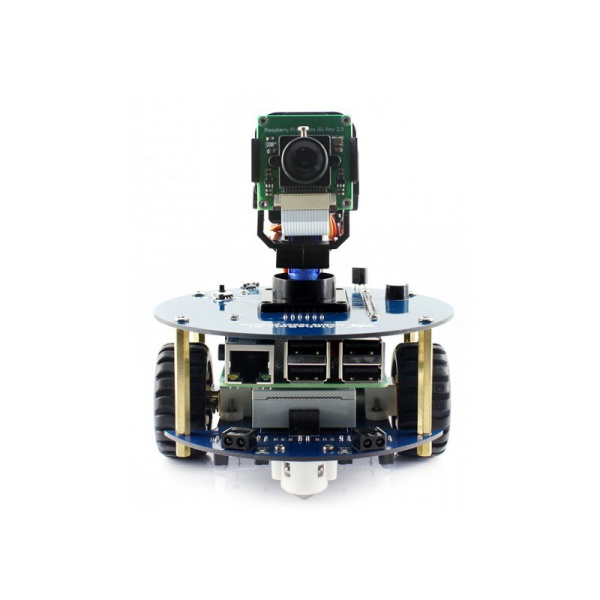
\includegraphics[width=7cm]{Alphabot2-pi-3.png}
    \caption{AlphaBot2 RPi assembled}
    \label{fig:fig1}
\end{figure}

The bottom board, which serves as the base of the robot, has different components that must be identified (Figure \ref{fig:fig2}).

\begin{figure}[H]
    \centering
    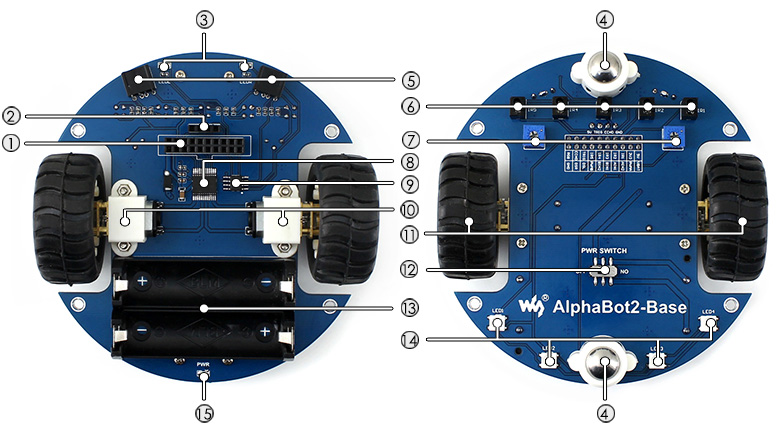
\includegraphics[width=9.50cm]{AlphaBot2-Base-intro.jpg}
    \caption{AlphaBot2 RPi base board}
    \label{fig:fig2}
\end{figure}

This board consists of the following components:

\begin{enumerate}
    \item Ultrasonic module interface
    \item AlphaBot2 control interface: for connecting sorts of controller adapter board
    \item Obstacle avoiding indicators
    \item Omni-direction wheel
    \item ST188: reflective infrared photoelectric sensor, for obstacle avoiding
    \item ITR20001/T: reflective infrared photoelectric sensor, for line tracking
    \item Potentiometer for adjusting obstacle avoiding range
    \item TB6612FNG dual H-bridge motor driver
    \item LM393 voltage comparator
    \item N20 micro gear motor reduction rate 1:30, 6V/600RPM
    \item Rubber wheels diameter 42mm, width 19mm
    \item Power switch
    \item Battery holder: supports 14500 batteries
    \item WS2812B: true color RGB LEDs
    \item Power indicator
\end{enumerate}

The connection to Raspberry Pi is made through the top board (Figure \ref{fig:fig3}).

\begin{figure}[H]
    \centering
    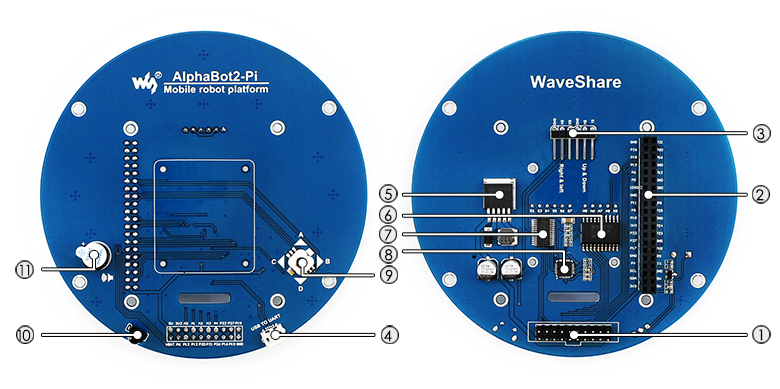
\includegraphics[width=9.50cm]{AlphaBot2-Pi-intro.jpg}
    \caption{AlphaBot2 RPi connection to Raspberry Pi}
    \label{fig:fig3}
\end{figure}

This board has the following components:

\begin{enumerate}
    \item AlphaBot2 control interface: for connecting AlphaBot2-Base
    \item Raspberry Pi interface: for connecting Raspberry Pi 3 Model B
    \item Servo interface
    \item USB TO UART: easy for controlling the Pi via UART
    \item LM2596: 5V voltage regulator
    \item TLC1543: 10-bit AD acquisition chip, allows the Pi to use analog sensors
    \item PCA9685: servo controller, make it more smoothly to rotate the pan head
    \item CP2102: USB TO UART converter
    \item Joystick
    \item IR receiver
    \item Buzzer
\end{enumerate}

\subsubsection{Simulated Robot Specification} \label{spec_sim}

For the construction of the simulated robot, we tried to use the real dimensions of the Alphabot2 RPi.

Since many robot components did not need to be simulated, only a robot with the chassis, sensors, wheels, casters and camera was created, where the positions of these components are the same as the positions they occupy in the real robot.

The whole simulated robot was implemented using an .xacro file that is executed in the Gazebo, in which only the chassis and the camera are represented through meshes and the remaining forms through geometries of the Gazebo.

Thus, this simulated robot will have 5 lower sensors, with a vertical scan to detect lines and 2 upper sensors with a range between -15 degrees and 15 degrees, making a total of 30 degrees and a minimum distance of 1cm and maximum of 15cm. For line detection sensors, the Gazebo plugin for a camera type sensor was used and for the obstacle detection was used the plugin that creates laser sensors.

The final look of the simulated robot can be visualized in Figure \ref{fig:fig4}.

\begin{figure}[H]
    \centering
    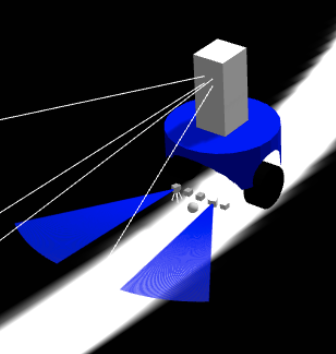
\includegraphics[width=7cm]{Simulated-robot.png}
    \caption{AlphaBot2 RPi simulated on Gazebo}
    \label{fig:fig4}
\end{figure}

\subsection{Robot Behaviour} \label{behaviour}

This robot follows a subsumption based architecture as the one shown in Figure \ref{fig:fig5}.

\begin{figure}[H]
    \centering
    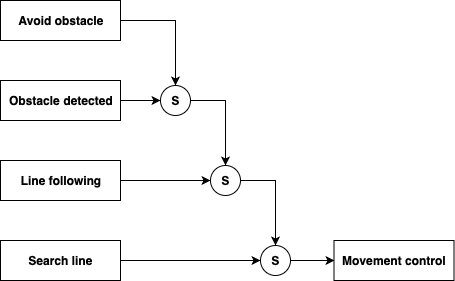
\includegraphics[width=8.5cm]{Subsumption.png}
    \caption{Subsumption based architecture}
    \label{fig:fig5}
\end{figure}

According to the architecture, the robot presents only four possible behaviors, being the first representative of the initial movement, the second one relative to the line following, the third related to obstacles detection and the fourth and last one related to the obstacles avoidance.

Initially, the robot moves itself around the map searching for a line (initial movement). As soon as the robot detects a line, it follows the line through an imaginary parallel line. 

Then, if the robot's sensors detect an obstacle it will assume another behaviour, in order to avoid the collision of the robot with that obstacle.

If the obstacle is to the left of the robot, it has to deviate from the right and vice versa. If the obstacle is in front of the robot it can deviate from either the left or the right.

\subsection{World} \label{world}

Initially, the world/track created for the simulated robot to be tested was an adaptation of the track used by Conde\cite{b1, b2, b3}.

Conde's track is an extensive track, with two carriage ways, a treadmill and traffic lights that indicated whether or not the robot could move forward. In addition, this lane could have some obstacles in its way, which the robot would have to avoid. Figure \ref{fig_fig6} represents the Conde's world.

\begin{figure}[H]
    \centering
    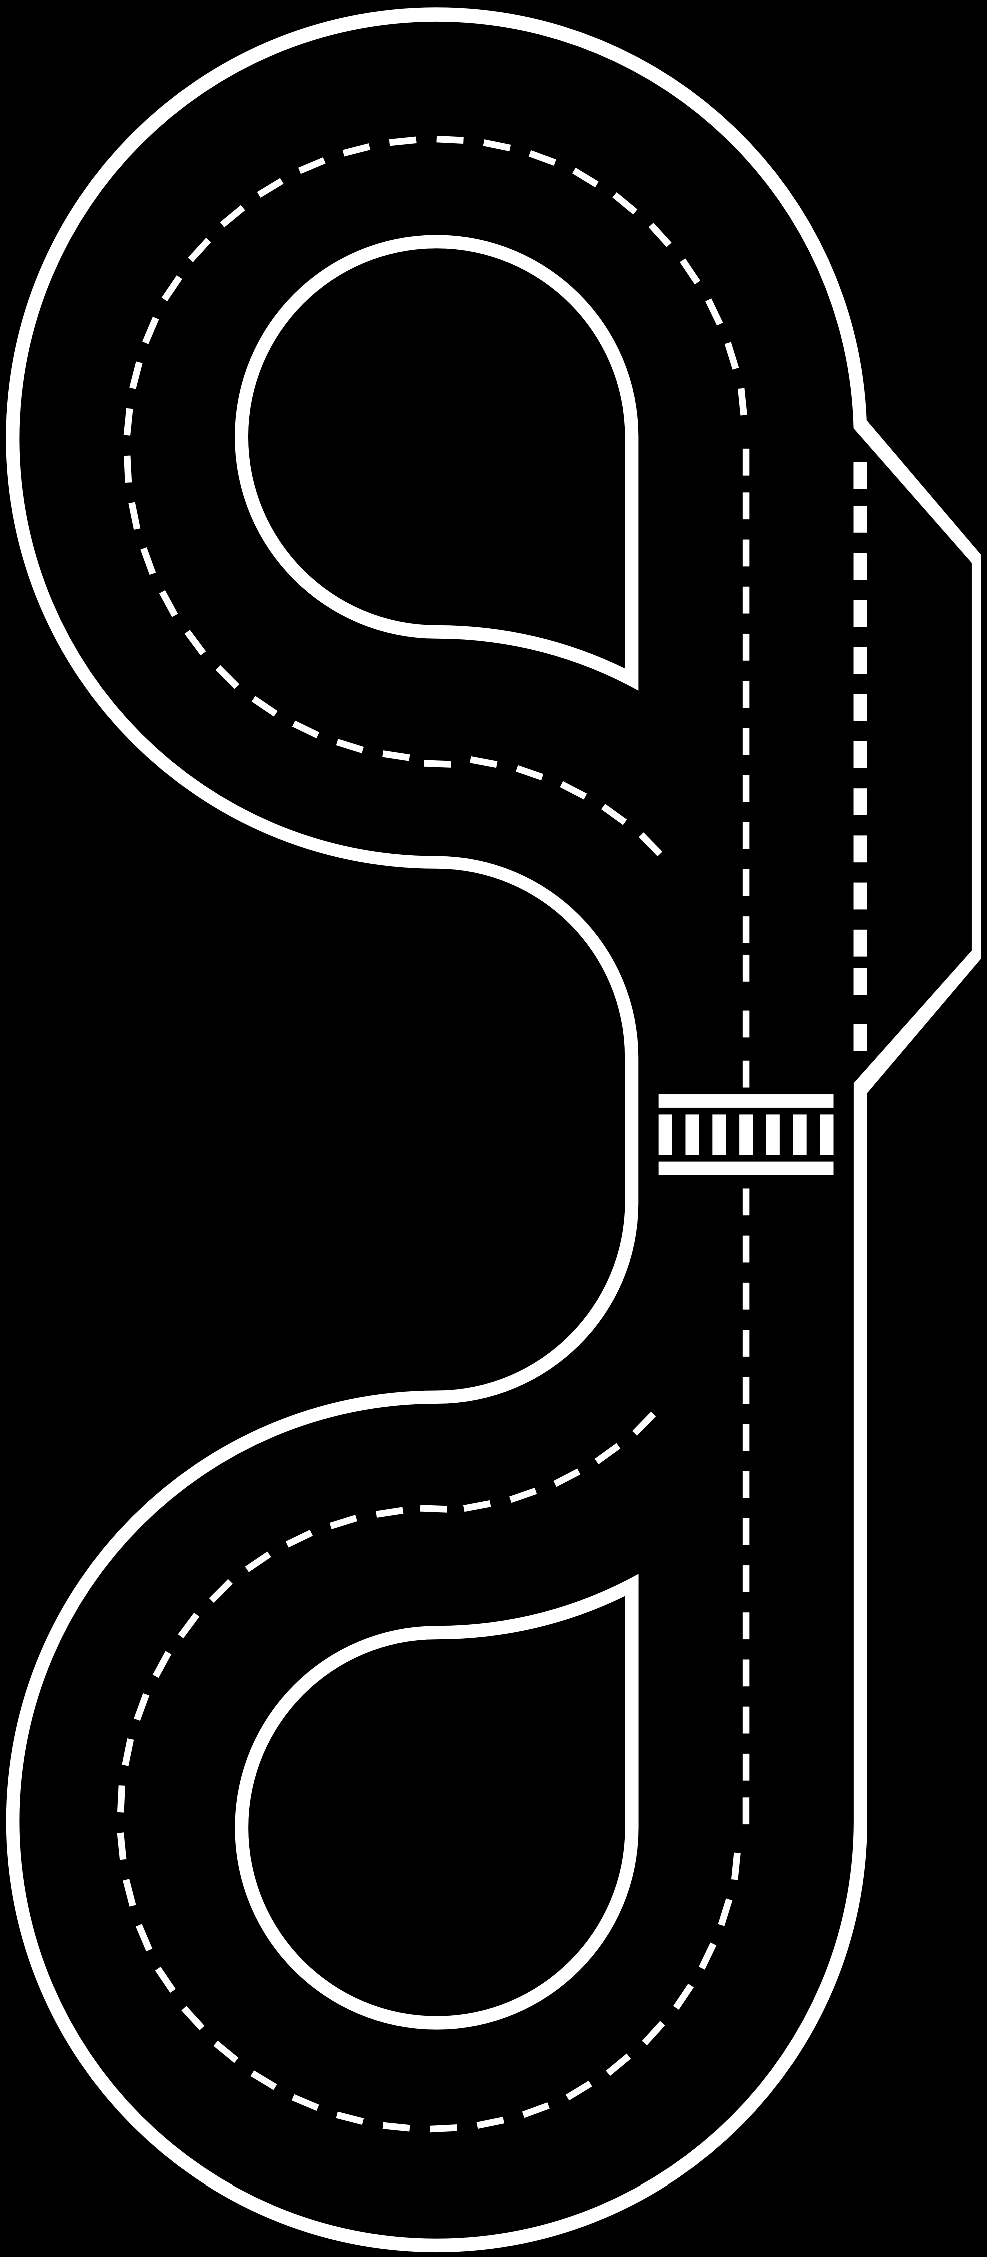
\includegraphics[width=2cm]{Conde-track.png}
    \caption{Conde's world}
    \label{fig:fig6}
\end{figure}

The track created for the AlphaBot2 RPi is therefore an adaptation of the Count's lane, since it only curtailed its entire path, keeping the treadmill, traffic lights and possible obstacles. Figure \ref{fig:fig7} shows the track adapted for the AlphaBot2 RPi.

\begin{figure}[H]
    \centering
    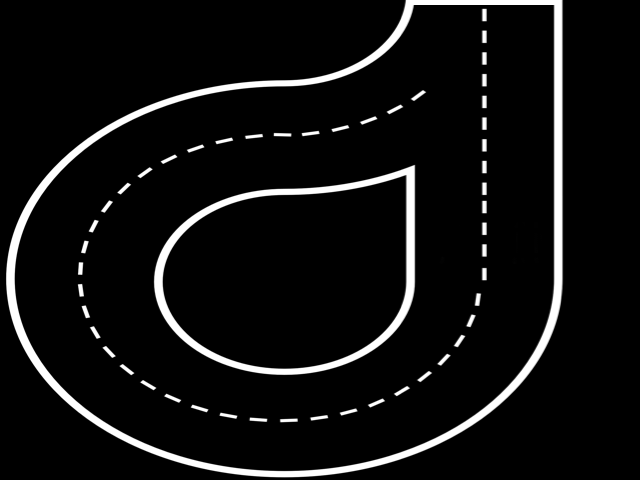
\includegraphics[width=3cm]{AB2-track.png}
    \caption{Alphabot2 RPi's world}
    \label{fig:fig7}
\end{figure}

Although this new track was created, a simpler track was created, just to test the robot's behavior (Figure \ref{fig:fig8}).

\begin{figure}[H]
    \centering
    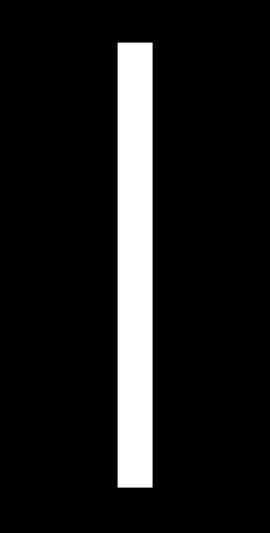
\includegraphics[width=3cm]{AB2-track2.png}
    \caption{Alphabot2 RPi's testing world}
    \label{fig:fig8}
\end{figure}


\subsection{Architecture} \label{ros}

Figure \ref{fig:fig9} represents the node architecture used so that it is possible to interconnect the real and simulated Alphabot2 RPi, allowing its movement and the fulfillment of the objectives of this activity.

\begin{figure}[H]
    \centering
    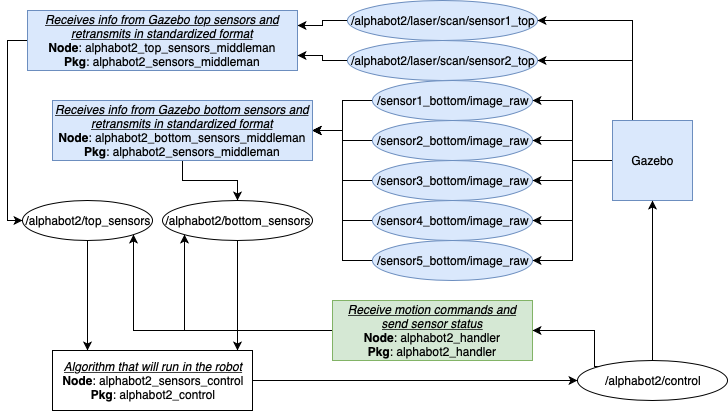
\includegraphics[width=9.5cm]{arch.png}
    \caption{Alphabot2 RPi architecture}
    \label{fig:fig9}
\end{figure}

\subsection{Approach} \label{alg}

In order for the real and simulated Alphabot2 RPi to achieve the desired goals, it was necessary to create different algorithms that would allow them to avoide obstacles and to follow lines.

Most of the code used by the real robot was taken from the demo code on the Alphabot2 website, so you can program both your software and your hardware. Even so, it was still necessary to change some details, namely the linear and angular velocity values, so that both the real and the simulated robot walked at equal speeds when searching for the line to follow or avoid obstacles.

\subsubsection{Ros Topics} \label{topics}

Firstly, we defined the different ROS topics where the sensors would publish the values they scanned.

The two upper sensors, represented by laser scanners, which detect obstacles, publish their results for the following topics:

\begin{itemize}
    \item ``/alphabot2/laser/scan/sensor1\_top''
    \item ``/alphabot2/laser/scan/sensor2\_top''
\end{itemize}

The five bottom sensors, represented by camera sensors to detect the lines' brightness, publish their results for the following topics:

\begin{itemize}
    \item ``/sensor1\_bottom/image\_raw''
    \item ``/sensor2\_bottom/image\_raw''
    \item ``/sensor3\_bottom/image\_raw''
    \item ``/sensor4\_bottom/image\_raw''
    \item ``/sensor5\_bottom/image\_raw''
\end{itemize}

These results will be subscribed on the side of the algorithms to be evaluated and later published for other ROS topics to be subscribed either by the real robot or by the simulated robot.

These new ROS topics will be described below.

\subsubsection{Obstacle Avoidance} \label{obs}

To detect obstacles, we first check whether the values read by the two upper sensors are infinite values. If these values were not infinite, it means that the sensors were able to detect an obstacle, by creating an array with two boolean values representing the detection of obstacles by each of the sensors, which would be published for the topic ``/alphabot2/top\_sensors'' (Figure \ref{fig:fig10}).

\begin{figure}[H]
    \centering
    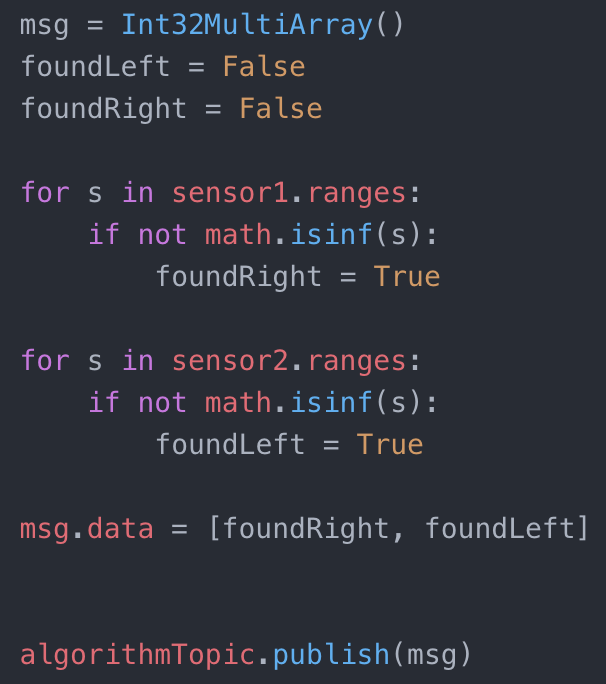
\includegraphics[width=5cm]{algorithm1.png}
    \caption{Top sensors analysis}
    \label{fig:fig10}
\end{figure}

After this initial analysis, each robot subscribes to the topic ``/alphabot2/top\_sensors'' and checks the values that were published there.

\textbf{If it turns out that the left sensor has a value of true, it means that there was an obstacle on the left and therefore the robot would have to turn right (with a minimal linear velocity of 0.2m/s and an angular velocity of -1m/s$^{2}$). If it turns out that the right sensor is true, it means that there was an obstacle on the right and that the robot would have to turn left (with a minimal linear velocity of 0.2m/s and an angular velocity of 1m/s$^{2}$). If none of these occur, the robot moves forward with its normal velocities (maximum linear velocity of 1m/s and angular velocity of 0.3m/s$^{2}$) (Figure \ref{fig:fig11})}.

\begin{figure}[H]
    \centering
    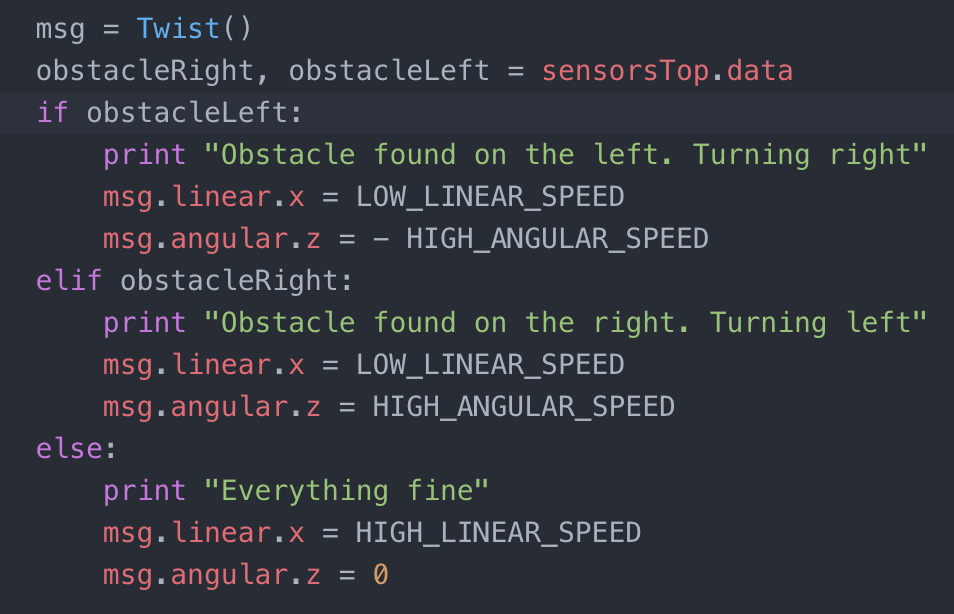
\includegraphics[width=7cm]{algorithm2.png}
    \caption{Top sensors' results analysis}
    \label{fig:fig11}
\end{figure}

\subsubsection{Line Following} \label{line}

To follow lines, we first calculate the brightness percentage scanned by the five bottom sensors, publishing them on the topic ``/alphabot2/bottom\_sensors'' (Figure \ref{fig:fig12}).

\begin{figure}[H]
    \centering
    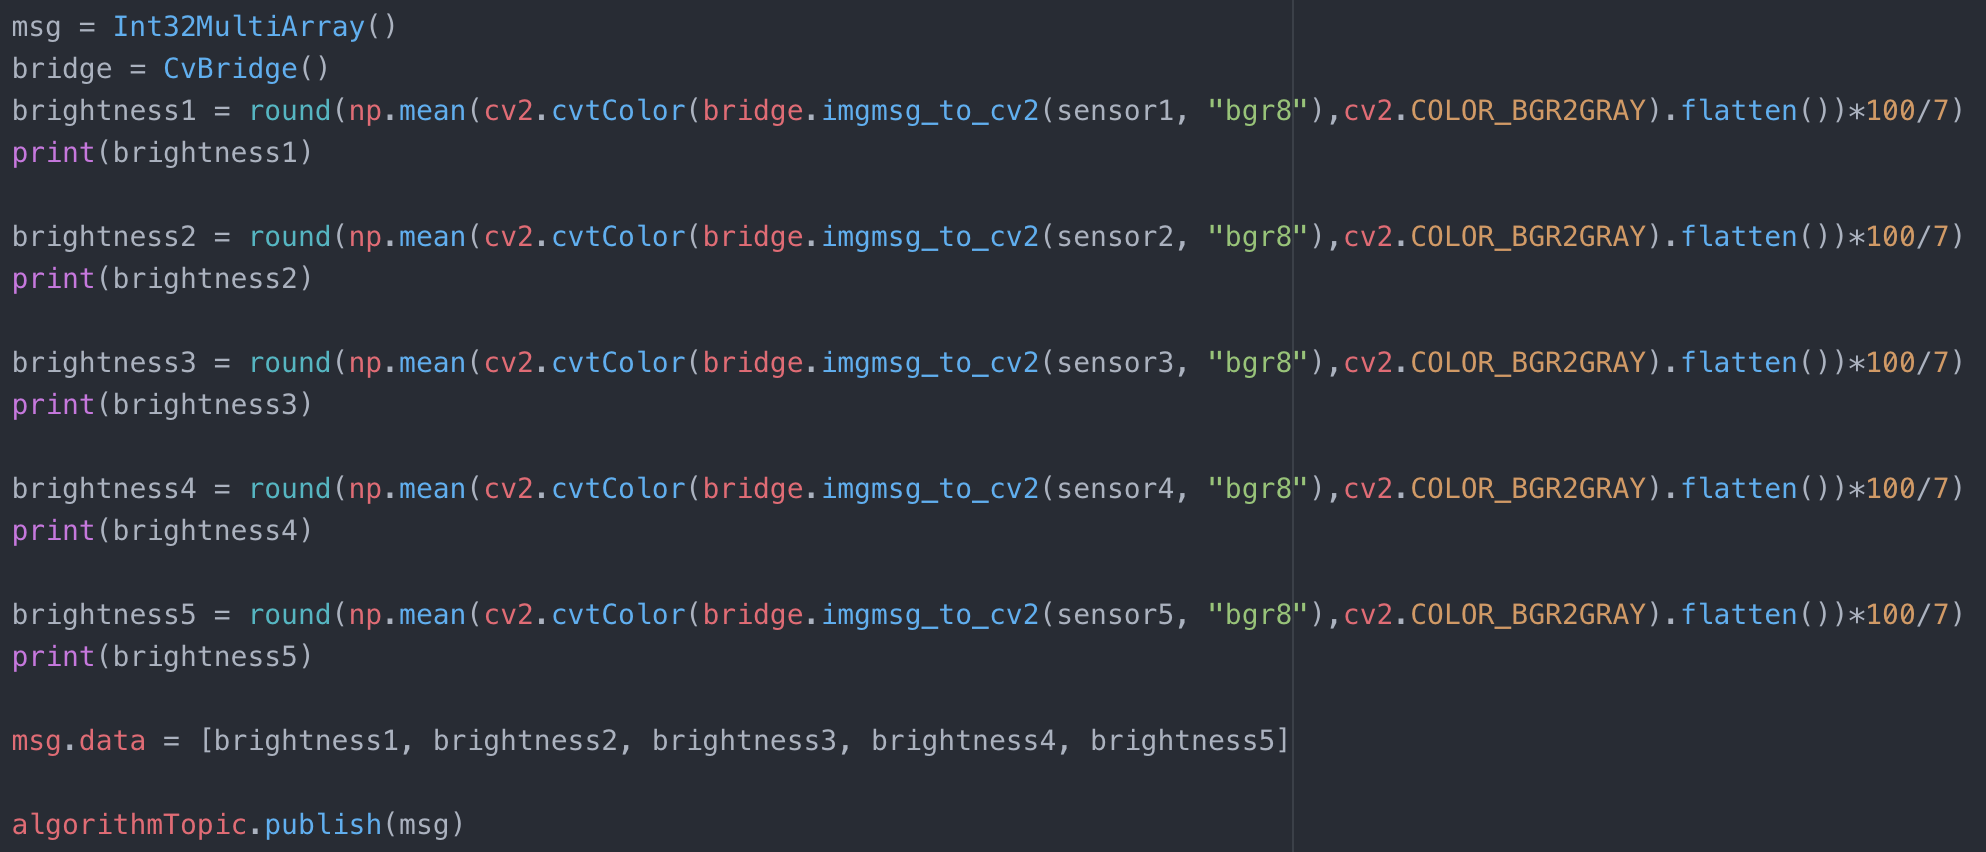
\includegraphics[width=9cm]{algorithm3.png}
    \caption{Bottom sensors brigthness analysis and calculations}
    \label{fig:fig12}
\end{figure}

After this initial analysis, each robot subscribes to the topic ``/alphabot2/bottom\_sensors'' and checks the bigthness values that were published there.

\textbf{If it turns out that the middle sensor scanned 100\% of brightness, it means that there was a line under it, having to be further captured 100\% brightness by one of the other 4 sensors. Therefore the robot moves forward with its normal velocities (maximum linear velocity of 1m/s and angular velocity of 0.3m/s$^{2}$). If the most right sensor scanned more brightness than the most left sensor, it means that the line is on the right side of the robot and it would have to turn right (with a minimal linear velocity of 0.2m/s and an angular velocity of -1m/s$^{2}$). If the most left sensor scanned more brightness than the most right sensor or the same value, it means that the line is on the left side of the robot and it would have to turn left (with a minimal linear velocity of 0.2m/s and an angular velocity of 1m/s$^{2}$) (Figure \ref{fig:fig13})}.

\begin{figure}[H]
    \centering
    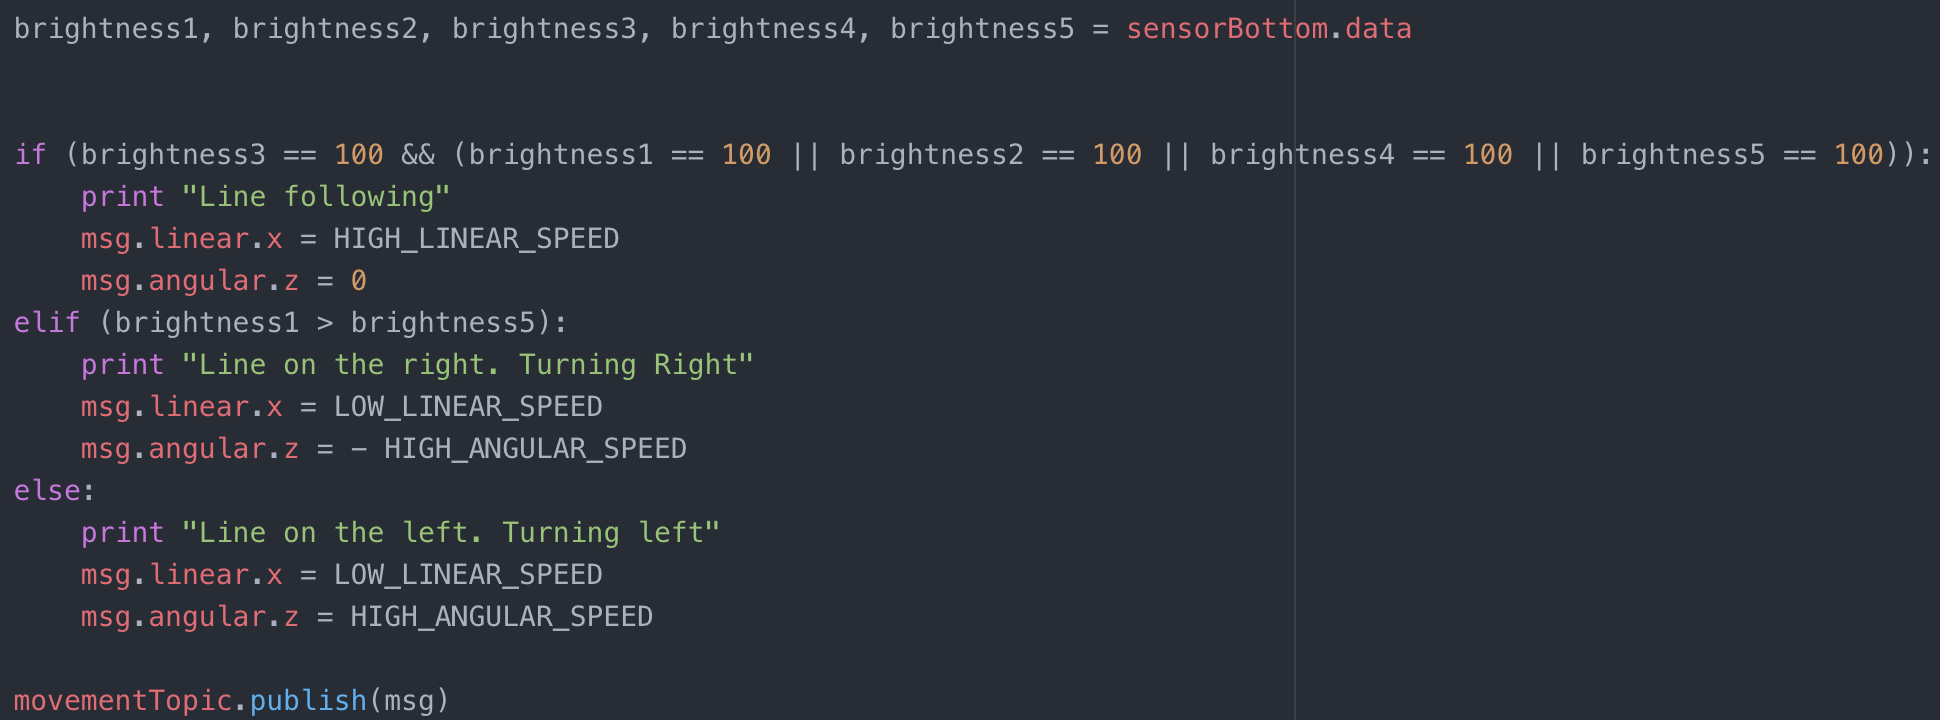
\includegraphics[width=9.5cm]{algorithm4.png}
    \caption{Bottom sensors' results analysis}
    \label{fig:fig13}
\end{figure}


\section{Results} \label{results}


\section{Conclusions} \label{conclusions}


\begin{thebibliography}{00}
\bibitem{b1} Costa, Valter, Peter Cebola, Armando Sousa, and Ana Reis. 2018. “Design Hints for Efficient Robotic Vision - Lessons Learned from a Robotic Platform.” Lecture Notes in Computational Vision and Biomechanics 27. Springer Netherlands: 515–24. doi:10.1007/978-3-319-68195-5\_56.
\bibitem{b2} Costa, Valter, Rosaldo Rossetti, and Armando Sousa. 2017. “Simulator for Teaching Robotics, ROS and Autonomous Driving in a Competitive Mindset.” International Journal of Technology and Human Interaction 13 (4): 19–32. doi:10.4018/IJTHI.2017100102.
\bibitem{b3} Bu, Yi, Binglu Wang, Win bin Huang, Shangkun Che, and Yong Huang. 2018. “Using the Appearance of Citations in Full Text on Author Co-Citation Analysis.” Scientometrics 116 (1). Springer Netherlands: 275–89. doi:10.1007/s11192-018-2757-z.
\bibitem{b4} Roy, Abhishek, and Mathew Mithra Noel. 2016. “Design of a High-Speed Line Following Robot That Smoothly Follows Tight Curves.” Computers and Electrical Engineering 56 (November). Elsevier Ltd: 732–47. doi:10.1016/j.compeleceng.2015.06.014.
\bibitem{b5} Matczak, Grzegorz, and Przemysław Mazurek. 2017. “Dim Line Tracking Using Deep Learning for Autonomous Line Following Robot.” In Advances in Intelligent Systems and Computing, 573:414–23. Springer Verlag. doi:10.1007/978-3-319-57261-1\_41.
\bibitem{b6} Javed, Mudassir, Sohail Hamid, Muhammad Talha, Zubair Ahmad, Fazle Wahab, and Hazrat Ali. 2018. “Input Based Multiple Destination, Multiple Lines Following Robot with Obstacle Bypassing.” ICST Transactions on Scalable Information Systems 5 (16): 154472. doi:10.4108/eai.13-4-2018.154472.
\bibitem{b7} Tanveer, M. Hassan, Carmine T. Recchiuto, and Antonio Sgorbissa. 2019. “Analysis of Path Following and Obstacle Avoidance for Multiple Wheeled Robots in a Shared Workspace.” Robotica 37 (1): 80–108. doi:10.1017/S0263574718000875.
\bibitem{b8} Matczak, Grzegorz, and Przemysław Mazurek. 2016. “Tracklet-Based Viterbi Track-Before-Detect Algorithm for Line Following Robots.” In , 649–58. doi:10.1007/978-3-319-26227-7\_61.
\bibitem{b9} 15th International Conference on Ubiquitous Robots, {UR} 2018, Honolulu, HI, USA, June 26-30, 2018. IEEE. 2018. Retrived from \url{http://ieeexplore.ieee.org/xpl/mostRecentIssue.jsp?punumber=8424588}. isbn:978-1-5386-6334-9.
\bibitem{b10} 3rd International Conference on Computing, Communication, Control and Automation (ICCUBEA-2017), August, 2017. IEEE. 2017. Retrived from \url{http://apps.webofknowledge.com/full_record.do?product=WOS&search_mode=GeneralSearch&qid=19&SID=E1Sb736VNEXNGjBndQd&page=5&doc=46&cacheurlFromRightClick=no}
\end{thebibliography}

\vspace{12pt}

\end{document}
